\iffalse
\chapter{2009}
\author{AI24BTECH11031}
\section{me}
\fi

\item For a matrix $\vec{M} = \myvec{\frac{3}{5} & \frac{4}{5} \\ x & \frac{3}{5}}$,
the transpose of the matrix is equal to the inverse of the matrix, $\vec{M}^\top = \vec{M}^{-1}$.
The value of $x$ is given by
\begin{multicols}{4}
\begin{enumerate}
    \item $-\frac{4}{5}$
    \item $-\frac{3}{5}$
    \item $\frac{3}{5}$
    \item $\frac{4}{5}$
\end{enumerate}
\end{multicols}

\item The divergence of the vector field $3xz\hat{i} + 2xy\hat{j} - yz^2\hat{k}$
at a point $\brak{1, 1, 1}$ is equal to
\begin{multicols}{4}
\begin{enumerate}
    \item 7
    \item 4
    \item 3
    \item 0
\end{enumerate}
\end{multicols}

\item The inverse Laplace transform of $\frac{1}{\brak{s^2 + s}}$ is
\begin{multicols}{4}
\begin{enumerate}
    \item $1 + e^t$
    \item $1 - e^t$
    \item $1 - e^{-t}$
    \item $1 + e^{-t}$
\end{enumerate}
\end{multicols}

\item If three coins are tossed simultaneously, the probability of getting at
least one head is
\begin{multicols}{4}
\begin{enumerate}
    \item $\frac{1}{8}$
    \item $\frac{3}{8}$
    \item $\frac{1}{2}$
    \item $\frac{7}{8}$
\end{enumerate}
\end{multicols}

\item If a closed system is undergoing an irreversible process, the entropy
of the system
\begin{enumerate}
    \item must increase
    \item always remains constant
    \item must decrease
    \item can increase, decrease or remain constant
\end{enumerate}

\item A coolant fluid at $30 \degree C$ flows over a heated flat plate
maintained at a constant temperature of $100 \degree C$. The boundary
layer temperature distribution at a given location on the plate may be
approximated as $T = 30 + 70\exp\brak{-y}$ where $y$ (in m) is the
distance normal to the plate and $T$ is in $\degree C$. If thermal
conductivity of the fluid is 1.0 $\frac{W}{mK}$, the local convective heat
transfer coefficient (in $\frac{W}{m^2K}$) at that location will be
\begin{multicols}{4}
\begin{enumerate}
    \item 0.2
    \item 1
    \item 5
    \item 10
\end{enumerate}
\end{multicols}

\item A frictionless piston-cylinder device contains a gas initially at
0.8 MPa and 0.015 $m^3$. It expands quasi-statically at constant
temperature to a final volume of 0.030 $m^3$. The work output (in kJ)
during this process will be
\begin{multicols}{4}
\begin{enumerate}
    \item 8.32
    \item 12.00
    \item 554.67
    \item 8320.00
\end{enumerate}
\end{multicols}

\item In an ideal vapour compression refrigeration cycle, the specific
enthalpy of refrigerant (in $\frac{kJ}{kg}$) at the following states is given as: \\
Inlet of condenser: 283 \\
Exit of condenser: 116 \\
Exit of evaporator: 232 \\
The COP of this cycle is
\begin{multicols}{4}
\begin{enumerate}
    \item 2.27
    \item 2.75
    \item 3.27
    \item 3.75
\end{enumerate}
\end{multicols}

\item A compressor undergoes a reversible, steady flow process. The gas
at inlet and outlet of the compressor is designated as state 1 and state
2 respectively. Potential and kinetic energy changes are to be ignored.
The following notations are used:

$v$ = specific volume and $P$ = pressure of the gas.

The specific work required to be supplied to the compressor for this gas
compression process is 
\begin{multicols}{4}
\begin{enumerate}
\item $\int_{1}^{2} Pdv$
\item $\int_{1}^{2} vdP$
\item $v_1\brak{P_2 - P_1}$
\item $-P_2\brak{v_1 - v_2}$
\end{enumerate}
\end{multicols}

\item A block weighing 981 N is resting on a horizontal surface. The coefficient
of friction between the block and the horizontal surface is $\mu = 0.2$. A vertical
cable attached to the block provides partial support as shown. A man can pull
horizontally with a force of 100 N. What will be the tension, $T$ (in N), in the
cable if the man is just able to move the block to the right?

\begin{center}
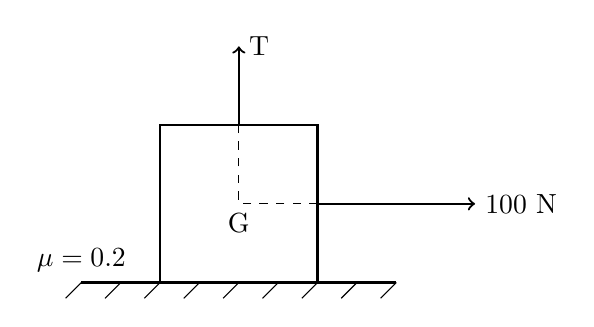
\begin{tikzpicture}
    \draw[thick] (0,0) rectangle (2,2); 
    \draw[thick] (-1, 0) node[above] {$\mu = 0.2$} -- (3, 0); 
    
    \foreach \i in {-2,...,6} {
        \draw (\i/2, 0) -- (\i/2-0.2, -0.2);
    }

    \draw[->, thick] (2,1) -- (4,1) node[right] {100 N};
    \draw[->, thick] (1,2) -- (1,3) node[right] {T};
    \draw[dashed] (2,1) -- (1,1) node[below] {G} -- (1,2);
\end{tikzpicture}
\end{center}

\begin{multicols}{4}
\begin{enumerate}
    \item 176.2
    \item 196.0
    \item 481.0
    \item 981.0
\end{enumerate}
\end{multicols}

\item If the principal stresses in a plane stress problem are $\sigma_1 = 100$ MPa,
$\sigma_2 = 40$ MPa, the magnitude of the maximum shear stress (in MPa) will be
\begin{multicols}{4}
\begin{enumerate}
    \item 60
    \item 50
    \item 30
    \item 20
\end{enumerate}
\end{multicols}

\item A simple quick return mechanism is shown in the figure. The forward to return
ratio of the quick return mechanism is $2:1$. If the radius of the crank $O_1P$ is
125 mm, then the distance $d$ (in mm) between the crank center to lever pivot center
point should be

\begin{center}    
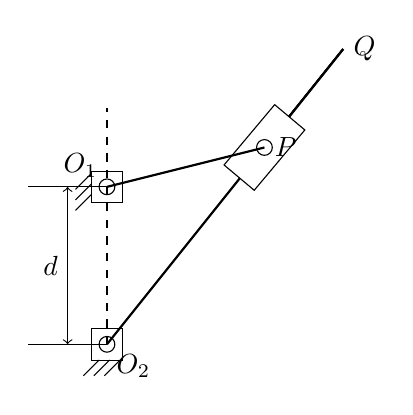
\begin{tikzpicture} 
    \draw (0,2) circle (0.1) node[above left] {$O_1$};
    \draw (0,0) circle (0.1) node[below right] {$O_2$};
    \draw (-0.2,0.2) rectangle (0.2,-0.2);
    \draw (-0.2,2.2) rectangle (0.2, 1.8);
    
    \foreach \i in {0,...,2} {
        \draw (\i*0.4/3-0.1, -0.2) -- (\i*0.4/3-0.3, -0.4);
        \draw (-0.2, 2+\i*0.4/3-0.1) -- (-0.4, 2+\i*0.4/3-0.3);
    }

    \draw[dashed] (0,0) -- (0,3); 
    \draw[<->] (-0.5,0) -- (-0.5,2) node[midway, left] {$d$};
    
    \draw (-1, 2) -- (0, 2);
    \draw (-1, 0) -- (0, 0);
    
    \draw[thick] (0,0) -- (3,3.75);
    \draw[thick] (2,2.5) -- (3,3.75) node[right] {$Q$};
    \filldraw[fill=white,rotate around={50:(2,2.5)}] (1.5,2.25) rectangle (2.5,2.75);
    \draw (2,2.5) circle (0.1);
    \draw[thick] (0,2) -- (2,2.5) node[right] {$P$};
\end{tikzpicture}
\end{center}

\begin{multicols}{4}
\begin{enumerate}
    \item 144.3
    \item 216.5
    \item 240.0
    \item 250.0
\end{enumerate}
\end{multicols}
